% -*- TeX-master: "main"; fill-column: 72 -*-

\newcommand{\fixttspace}{\hspace*{1pt}}

\section{Package syntax and semantics}

In this section, we define the syntax and semantics of the Hierarchical
Model Composition package for SBML Level~3 Version~1.  We expound on the
various data types and constructs defined in this package, then in
\sect{examples}, we provide complete examples of using the constructs in
example SBML models.

\subsection{Namespace URI and other declarations necessary for using this package}
\label{xml-namespace}

Every SBML Level~3 package is identified uniquely by an XML namespace
URI.  For an SBML document to be able to use a given SBML Level~3
package, it must declare the use of that package by referencing its URI.
The following is the namespace URI for this version of the Qualitative Models package for SBML Level~3 Version~1:
\begin{center}
\uri{http://www.sbml.org/sbml/level3/version1/qual/version1}
\end{center}

In addition, SBML documents using a given package must indicate whether
understanding the package is required for complete mathematical
interpretation of a model, or whether the package is optional.  This is
done using the attribute \token{required} on the \token{<sbml>} element
in the SBML document.  For the Qualitative Models package,
the value of this attribute must be set to \val{true}.

The following fragment illustrates the beginning of a typical SBML model
using SBML Level~3 Version~1 and this version of the Qualitative Models package:

\begin{example}
<?xml version="1.0" encoding="UTF-8"?>
<sbml xmlns="http://www.sbml.org/sbml/level3/version1/core" level="3" version="1"
      xmlns:qual="http://www.sbml.org/sbml/level3/version1/qual/version1" qual:required="true">
\end{example}
    

% -----------------------------------------------------------------------------
\subsection{Primitive data types}
\label{primitive-types}

Section~3.1 of the SBML Level~3 specification defines a number of
primitive data types and also uses a number of XML Schema 1.0 data
types NEED CITATION.  We assume and use some of them in the rest of
this specification, specifically \primtype{boolean}, \primtype{ID},
\primtype{SId}, \primtype{SIdRef}, \primtype{UnitSId},
\primtype{UnitSIdRef}, and \primtype{string}. The Qualitative Model package defines other primitive types;
they are described below.

% removed for now
%\subsubsection{Type \fixttspace\primtypeNC{temporisationType}}
%\label{primtype-temporisation}
%
%The \primtype{temporisationType} is an enumeration of values used to indicate the updating policy used by %a \Transition.  The possible values are \const{timer}, \const{priority}, \const{sustain}, \const{proportion} %and \const{rate}.
%
\subsubsection{Type \fixttspace\primtypeNC{sign}}
\label{primtype-sign}

The \primtype{sign} is an enumeration of values used to indicate direction of an \Input within the system.  The possible values are \const{positive}, \const{negative}, \const{dual} and \const{unknown}.

\subsubsection{Type \fixttspace\primtypeNC{transitionInputEffect}}
\label{primtype-inputeffect}
The \primtype{transitionInputEffect} is an enumeration of values used to indicate the effect of an \Input \Transition within the system.  The possible values are \const{none} and \const{consumption}.

\subsubsection{Type \fixttspace\primtypeNC{transitionOutputEffect}}
\label{primtype-outputeffect}
The \primtype{transitionOutputEffect} is an enumeration of values used to indicate the effect of an \Output \Transition within the system.  The possible values are \const{production}, and \const{assignmentLevel}.

% -----------------------------------------------------------------------------
\subsection{Qualitative modelling}
\label{qual}

Before describing the classes and their attributes that have been used by this Qualitative Models Specification it is worth clarifying the intended meaning of some of the terms used. 

\subsubsection{Levels and symbols}

\TODO{need to address the issue of still allowing symbols in a simple form}

The entities being modelled have a \emph{level} associated with them that indicate the current state of the entity. 

A \emph{level} may be a boolean but may also represent more than two states and thus is considered to be an integer. In the case of the entity being a boolean its allowed levels would be \val{0} or \val{1}; but in other cases it may have any number of levels i.e. integer values up to and including a maximum. 

%A \emph{symbol} is intended to represent any value that might be appropriate in the model.  A user can %merely define the set of symbols that might be used and how the \token{symbolValue} associated with an %entity might be altered  by the model. 


\subsubsection{Transitions}

Qualitative Models consider \emph{transitions} between the levels/symbols of the entities involved in the model. This may involve the level of an entity being increased or decreased by a fixed amount; the level/symbol remaining unchanged; or the level/symbol being reassigned to an alternate value. Transitions occur when a set of conditions is met. These conditions may involve the levels/symbols falling above or below  a given \emph{threshold}. A simple example of this is the case where there are two entities A and B and the model states that when the level of A exceeds \val{1} (the threshold), the level of B is increased by \val{1}. 

\subsubsection{FunctionTerms}

The resulting value of an entity following a transition may have several possibilities that are governed by a number of conditions. Each transition can have a list of conditional functions \emph{functionTerms}, each associated with a result that allow the user to specify sets of piecewise conditions. For example a model may wish to encode the following

\begin{center}
$B = \left\{ \begin{array}{cc}
      B+1 & \mbox{if $A < 1$} \\
      B & \mbox{if $1 <= A < 3$} \\
     B + 2 & \mbox{otherwise}  \\
     \end{array}
\right.
$
\end{center}

In this case the \Transition would have a \FunctionTerm for each of the first two conditions and a \DefaultTerm for the otherwise component.





% -----------------------------------------------------------------------------
\subsection{The extended \class{Model} class}
\label{model-class}

The extension of SBML Level~3 Core's \Model class is relatively
straightforward: the Qualitative Models Package adds two lists,
one for holding qualitativeSpecies (\token{listOfQualitativeSpecies}, of class
\ListOfQualitativeSpecies), and the other for holding transitions (\token{listOfTransitions},
of class \ListOfTransitions).  \fig{qual-extended-model-uml} provides the UML
diagram.  The \sbml{Model} element may contain at most one \ListOfQualitativeSpecies, which must contain at least one \QualitativeSpecies. It may also contain at most one \ListOfTransitions which must contain at least one \Transition.The \QualitativeSpecies class and
the \Transition  class are defined in \sect{qualSpecies-class} and \sect{transitions-class} respectively.

\begin{figure}
  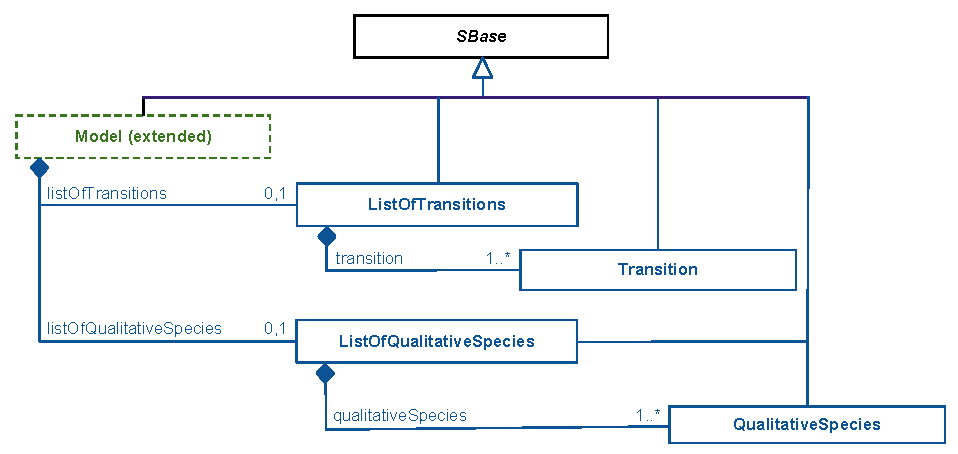
\includegraphics{figs/qual-extended-model-uml.pdf}
  \caption{The definitions of the extended \Model class. In other respects, \Model remains defined as
    in the SBML Level~3 Core specification.}
  \label{qual-extended-model-uml}
\end{figure}


% -----------------------------------------------------------------------------
\subsection{The \class{QualitativeSpecies} class}
\label{qualSpecies-class}
Similarly to the \sbml{Species} in SBML, the components of qualitative models refer to pools of entities that are considered indistinguishable and are each located in a specific \sbml{Compartment}. However, here components are characterised by their qualitative influences rather than by taking parts into reactions. Therefore, we define the \QualitativeSpecies element to represent such pools of entities.

A \QualitativeSpecies describes a pool of indistinguishable entities in a \sbml{Compartment}. It is associated with either a \token{level} or a \token{symbolValue} from its \ListOfSymbolicValues. These objects classes are defined in \fig{qual-qualitative-species-uml}.
\TODO{add listOfSymbols back}
\begin{figure}
  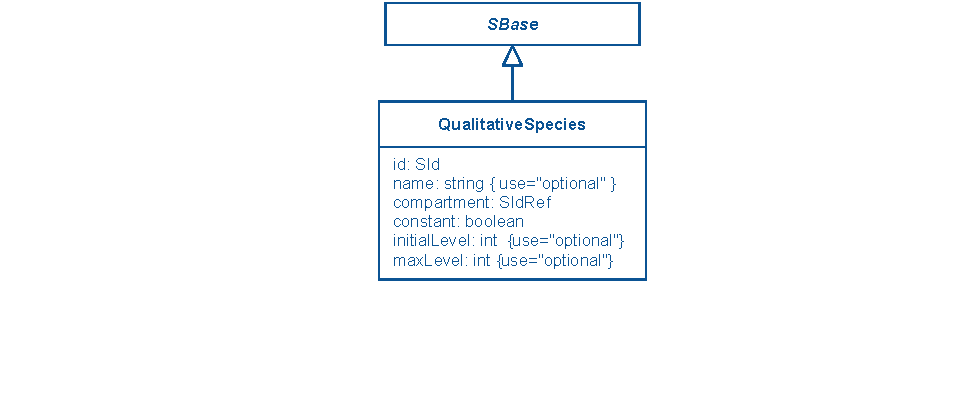
\includegraphics{figs/qual-qualitative-species-uml.pdf}
  \caption{The definitions of the \QualitativeSpecies class. }
  \label{qual-qualitative-species-uml}
\end{figure}

\paragraph{The \fixttspace\token{id} attribute}

The \token{id} attribute takes a required value
of type \primtype{SId}. The \token{id} is used as an identifier for the particluar \QualitativeSpecies. It can be used as a 
<ci> element within MathML, in which case it it interpreted as the \emph{level} or \emph{symbol} of this \QualitativeSpecies.

\paragraph{The \fixttspace\token{name} attribute}

A \QualitativeSpecies also has an optional \token{name} attribute of type \primtype{string}. 
 The \token{name} attribute should be used
in the same manner as on SBML Level~3 Core
objects; see Section~3.3.2 of the SBML Level~3 Version~1 Core
specification for more information.


\paragraph{The \token{compartment} attribute}
The required attribute \token{compartment}, of type \primtype{SIdRef}, is used to identify the compartment in which the qualitativeSpecies is located.  The attribute's value must be the identifier of an existing \sbml{Compartment} object in the model.  This attribute is comparable with the \token{compartment} attribute on the \sbml{Species} element.

\paragraph{The \token{constant} attribute}
The required attribute \token{constant}, of type \primtype{boolean}, is used to indicate that the \token{level} of the qualitativeSpecies is fixed or can be varied. This attribute is comparable with the \token{constant} attribute on the \sbml{Species} element.

\Q{If constant=true can the QS be an Input/Output or neither?}


\paragraph{The \token{initialLevel}  attribute}
The \token{initialLevel} is an \primtype{integer} that defines the initial \emph{level} of the \QualitativeSpecies in its \sbml{Compartment}. This attribute is optional.

\paragraph{The \token{maxLevel} attribute}
The \token{maxLevel} is an \const{integer} that sets the maximal \emph{level} of the \qualt{QualitativeSpecies}. This attribute is optional.

%\subsubsection{The \class{SymbolicValue} class}
%The \QualitativeSpecies element may contain at most one \ListOfSymbolicValues that contains zero or more %\SymbolicValue elements. An empty list is allowed, and useful for e.g. adding annotations.
%
%The \SymbolicValue element defines a non instantiated parameter that allows the model to associate %undefined values with a particular \QualitativeSpecies.
%Symbols can be considered as uninstantiated parameters. Such symbols may represent the different %solutions of piecewise linear differential equations, along with different thresholds.
%
%\paragraph{The \token{id} attribute}
%A \SymbolicValue element has an \token{id} attribute that takes a required value
%of type \primtype{SId}. The \token{id} is used as an identifier for the particluar \SymbolicValue and may be %referenced by the \token{symbolicResult} attribute of a \FunctionTerm within a \Transition to indicate that %this \SymbolicValue is the resulting value for this \QualitativeSpecies following a particular \Transition.
%
%\paragraph{The \token{name} attribute}
%There is an optional \token{name} attribute of type \primtype{string} that should be used
%in the same manner as on SBML Level~3 Core
%objects; see Section~3.3.2 of the SBML Level~3 Version~1 Core
%specification for more information.
%
%
%\paragraph{The \token{rank} attribute}
%The \token{rank} is an \primtype{integer} that defines the position of the symbol in the \ListOfSymbolicValues. This attribute is optional. \Q{What difference does the position make or does rank meaning ordering independent of physical position ?}
%
%\Q{Are symbols and levels exclusive?}



% -----------------------------------------------------------------------------
\subsection{The \class{Transition} class}
\label{transitions-class}
A \Transition element contains at most one \ListOfInputs and exactly one \ListOfOutputs and one \ListOfFunctionTerms. These objects classes are defined in \fig{qual-transition-uml}.

\begin{figure}
  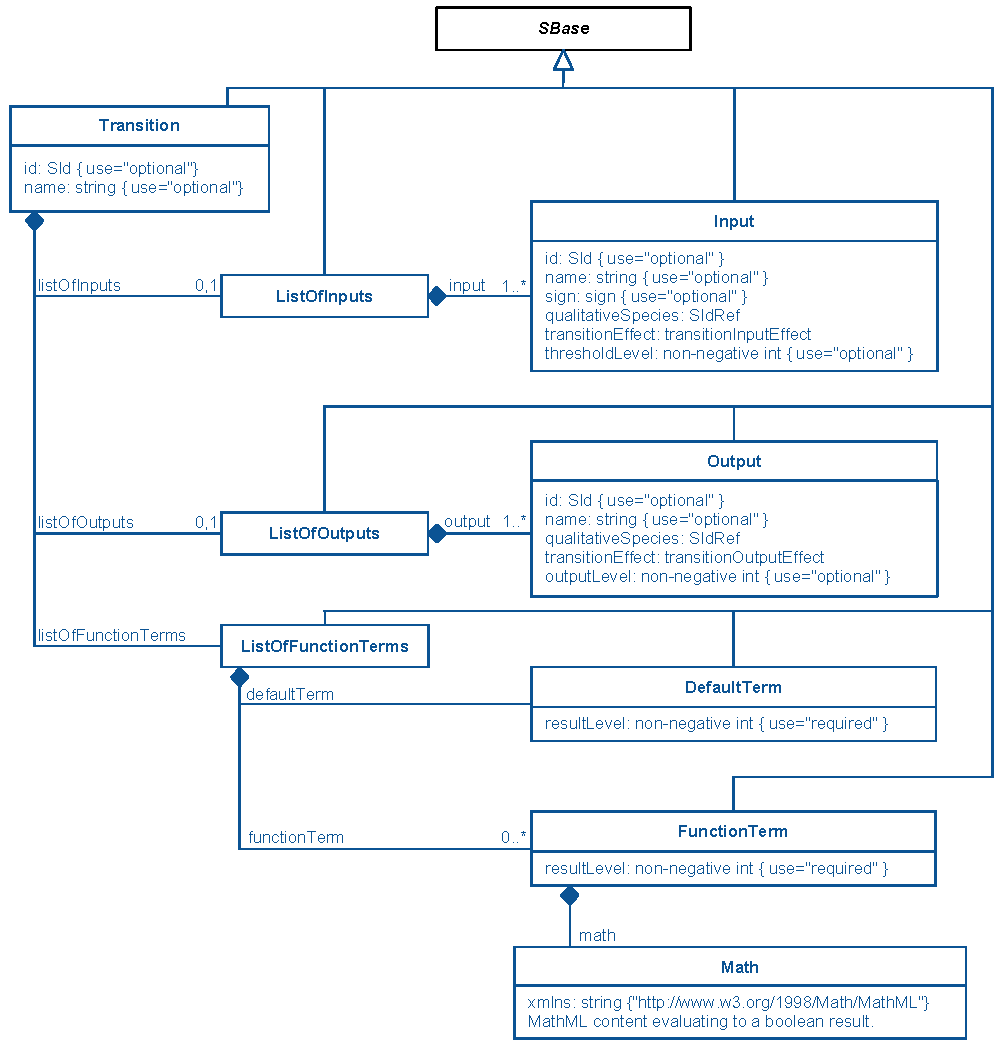
\includegraphics{figs/qual-transition-uml.pdf}
  \caption{The definitions of \Transition, \Input, \Output, \DefaultTerm and \FunctionTerm classes. Note that the \DefaultTerm class is not derived from SBase. }
  \label{qual-transition-uml}
\end{figure}

\paragraph{The \token{id} attribute}
A \Transition element has an optional \token{id} attribute of type \primtype{SId}. 

\paragraph{The \token{name} attribute}
There is an optional \token{name} attribute of type \primtype{string} that should be used
in the same manner as on SBML Level~3 Core
objects; see Section~3.3.2 of the SBML Level~3 Version~1 Core
specification for more information.

%\paragraph{The \token{temporisationType} attribute}
%A \Transition has an attribute \token{temporisationType} of type \primtype{temporisationType} used to indicate the updating policy associated with this \Transition element. This attribute is optional. \tab{transition-temporisation} describes the different updating policies.
%
%\begin{table}[thb]
%  \begin{edtable}{tabular}{p{1in}p{5in}}
%    \toprule
%    \textbf{TemporisationType} & \textbf{Interpretation} \\
%    \midrule
%    \const{timer} & TBD \\
%    \const{priority} & TBD \\
%    \const{sustain} & TBD \\
%    \const{proportion} & TBD \\
%    \const{rate} & TBD \\
%    \bottomrule
%  \end{edtable}
%  \caption{Interpretation of the \token{temporisationType} attribute on a \Transition.} 
%  \label{transition-temporisation}
%\end{table}
%
%\TODO{need more explanation of this}

\subsubsection{The \class{Input} class}
The \ListOfInputs contains zero or more elements of type \Input. A transition with zero inputs can be useful for defining an initial assignment, where the state of an output depends on a function but not on any input values. An empty list is allowed, and useful for e.g. adding annotations.
Each \Input refers to a \QualitativeSpecies that participates in the corresponding \Transition.

\paragraph{The \token{id} attribute}
An \Input element has an optional \token{id} attribute of type \primtype{SId}. The identifier of an \Input can be used as a 
<ci> element within MathML, in which case it it interpreted as the \token{thresholdLevel} or \token{thresholdSymbol}.

\paragraph{The \token{name} attribute}
There is an optional \token{name} attribute of type \primtype{string} that should be used
in the same manner as on SBML Level~3 Core
objects; see Section~3.3.2 of the SBML Level~3 Version~1 Core
specification for more information.


\paragraph{The \token{qualitativeSpecies} attribute}
The required attribute \token{qualitativeSpecies}, of type \primtype{SIdRef}, is used to identify the \QualitativeSpecies that is the \emph{input} of this \Transition.  The attribute's value must be the identifier of an existing \QualitativeSpecies object in the model.  This attribute is comparable with the \token{species} attribute on the \sbml{SpeciesReference} element.

\paragraph{The \token{thresholdLevel}  attribute}
The \token{thresholdLevel} is a \primtype{integer} that can be used to set the threshold level of the particular input.

\TODO{ Example}

\paragraph{The \token{transitionEffect} attribute}
Each \Input has a required attribute \token{transitionEffect} of type \primtype{transitionInputEffect} which describes how the \QualitativeSpecies referenced by the \Input is affected by the \Transition. \tab{transition-input} shows the possible values with the interpretation of each value.

\begin{table}[thb]
  \begin{edtable}{tabular}{p{1in}p{5in}}
    \toprule
    \textbf{TransitionInputEffect} & \textbf{Interpretation} \\
    \midrule
    \const{none} & Neither the level nor the symbol associated with the \token{qualitativeSpecies} is modified.\\
    \const{consumption} & The level of the \token{qualitativeSpecies} is decreased by the \token{resultLevel} of the selected term possibly modified by the \token{thresholdLevel} of the \Input.\\
    \bottomrule
  \end{edtable}
  \caption{Interpretation of the \token{transitionEffect} attribute on an \Input.} 
  \label{transition-input}
\end{table}

The following example illustrate the interpretation of the transitionEffect attribute. In the case of qualitativeSpecies \val{A} the \token{level} is unaltered by the `
\Transition. However the \token{level} of qualitativeSpecies \val{B} is reduced by \token{resultLevel} from the whichever \FunctionTerm is applicable (see Section|\ref{sec:function-term}

\begin{example}
<listOfInputs>
    <input qualitativeSpecies="A" thresholdLevel="1" transitionEffect="none"/>
    <input qualitativeSpecies="A" transitionEffect="consumption"/>
</listOfInputs>
\end{example}

\TODO{An example of a resultLevel modified by a thresholdLevel}
 
\paragraph{The \token{sign} attribute}
The \token{sign} of type \primtype{sign} can be used as an indication as to whether the contribution of this input is positive, negative, or both. The sign is usually used for visualization purposes only. This attribute is optional.


\subsubsection{The \class{Output} class}
The \ListOfOutputs contains at least one \Output.
Each \Output refers to a \QualitativeSpecies that participates in the corresponding \Transition.

\paragraph{The \token{id} attribute}
An \Output element has an optional \token{id} attribute of type \primtype{SId}. 

\paragraph{The \token{name} attribute}
There is an optional \token{name} attribute of type \primtype{string} that should be used
in the same manner as on SBML Level~3 Core
objects; see Section~3.3.2 of the SBML Level~3 Version~1 Core
specification for more information.



\paragraph{The \token{qualitativeSpecies} attribute}
The required attribute \token{qualitativeSpecies}, of type \primtype{SIdRef}, is used to identify the \QualitativeSpecies that is the \emph{output} of this \Transition.  The attribute's value must be the identifier of an existing \QualitativeSpecies object in the model.  This attribute is comparable with the \token{species} attribute on the \sbml{SpeciesReference} element.

\paragraph{The \token{outputLevel} attribute}
The \token{outputLevel} is an \primtype{integer} used along with the \token{transitionEffect} set to \const{production} to specify the effect of the \Transition on the corresponding \QualitativeSpecies. This attribute is optional. 
\Q{This contradicts the table}

\paragraph{The \token{transitionEffect} attribute}
Each \Output has a required attribute \token{transitionEffect} of type \primtype{transitionOutputEffect} which describes how the \QualitativeSpecies referenced by the \Output is affected by the \Transition. \tab{transition-output} shows the possible values with the interpretation of each value.

\begin{table}[thb]
  \begin{edtable}{tabular}{p{1in}p{5in}}
    \toprule
    \textbf{TransitionInputEffect} & \textbf{Interpretation} \\
    \midrule
    \const{production} & The level of the \token{qualitativeSpecies} is increased by the \token{resultLevel} of the selected term possibly modified by the \token{thresholdLevel} of the \Output.\\
    \const{assignmentLevel} & The level of the \token{qualitativeSpecies} is set to the \token{resultLevel} of the selected term. \\
%    \const{assignmentSymbol} & The symbol of the \token{qualitativeSpecies} is set to the \token{resultSymbol} of the selected term.\\
    \bottomrule
  \end{edtable}
  \caption{Interpretation of the \token{transitionEffect} attribute on an \Output.} 
  \label{transition-output}
\end{table}

\subsubsection{The \ListOfFunctionTerms class}

The \ListOfFunctionTerms may contain any number of \FunctionTerm elements, and exactly one \DefaultTerm.  Each \FunctionTerm encodes the conditions under which this term is selected.  The \DefaultTerm describes the results of the \Transition applied by default. The disjunction of the terms defines the \emph{qualitative function} associated with a \Transition.

\subsubsection{The \DefaultTerm class}
The \DefaultTerm defines the default result of a \Transition. 

\paragraph{The \token{resultLevel} attribute}
The default result is described by a \token{resultLevel}. This attribute is required.

The \token{resultLevel} is an \primtype{integer} describing a level. 

\Q{why is this not derived from SBase - since this means you cannot add an annotation to it}

\subsubsection{The \class{FunctionTerm} class}
\label{sec:function-term}

Each \FunctionTerm is also associated with a result (symbolic or level) and in addition to a Boolean function inside a \sbml{Math} element that can be used to set the conditions under which this term is selected.

\paragraph{The \token{resultLevel} and \token{resultSymbol} attributes}
The result of the term is described by a \token{resultLevel} or a \token{resultSymbol}. Both are optional, but one of them must be defined.

The \token{resultLevel} is an \primtype{integer} describing a level. The \token{resultSymbol} is a \primtype{SIdRef} referring to a \SymbolicValue.

\paragraph{The \sbml{Math} element:}
Each \qual{FunctionTerm} holds a Boolean function encoded in a \sbml{Math} element, using the subset of MathML 2.0 as defined in SBML L3v1 Section 3.4.6.
This element encodes the conditions under which the \FunctionTerm is selected.

%\paragraph{The \token{temporisationValue} attribute and the \sbml{TemporisationMath} element:}
%The attribute \token{temporisationValue} and the element \sbml{TemporisationMath} allow the specification of the "temporisation" of the \Transition under the corresponding \qual{FunctionTerm}. Both are optional. Depending on the value of the \token{temporisationType}, either one or both could be used.
%
%The \token{temporisationValue} is a \primtype{double}. The element \sbml{TemporisationMath} holds a MathML function returning a \primtype{double}. 


